\section{Applications}
\label{sec:applications}
\CRI{I suspect this section will have to go for EuroSec (and be condensed as a couple
of examples in the intro.)}

Efficient metadata tracking enables a wide range of valuable instrumentation
tools to be used with production systems where performance overhead is a
key characteristic. In the following we present a couple of key examples 
of such instrumentation.
% and their design relative to \projectname{}. 
This list is by no means exhaustive and we hope that readers
find other innovative uses of the framework. In this (short) paper, the applications  serve as motivation for our work and we will focus our evaluation on the framework itself.

\subsection{Write Integrity Protection}

Recent developments in attack techniques~\cite{carlini2015control,evans2015control,schuster2015counterfeit}
show the need to enforce additional data 
integrity within the program besides the classic control-flow integrity. 
Both Microsoft's WIT~\cite{akritidis2008preventing} and Oracle Application Data Integrity have looked into the 
topic of restricting the target addresses of memory writes using a coloring mechanism. 
In these schemes each memory location is associated with a given color and the instrumentation
alongside each memory write checks if the target location matches the color of
the pointer/instruction.
The major difference between the two schemes is the availability
of pointer color in the Oracle implementation stemming from a custom extension in
their latest CPU design. Microsoft on the other hand computes static colors for
the instruction based on points-to analysis.
In the case of both of these systems, the color for the memory location is tracked
using metadata shadowing with a fixed compression ratio.
Replacing these systems with \projectname{} can lead to substantial improvements  in  allocation performance.

In the case of both of these systems, the color for the memory location is tracked
using metadata shadowing with a fixed compression ratio. Thus integrating \projectname{}
into these systems is trivial, bringing with it all the advantages of variable compression ratio,
namely lower memory overhead and lower allocation overhead. However it does introduce
overhead when retrieving the metadata as the metadata information also needs to
be retrieved for the memory page corresponding to the pointer. In practice Write Integrity Protection
requires the most frequent metadata retrieval out of all the presented applications, showcasing the
worst case behaviour of \projectname{}.
\begin{comment}
To measure the effects of integrating \projectname{} into these systems, we
reimplemented the Microsoft scheme in a simplified manner. We use the DSA inter-procedural
points-to analysis~\cite{lattner2007making} from LLVM to identify connections between instructions
and memory locations. Since we only care about the performance characteristics of the metadata
tracking component, the accuracy of DSA relative to the points-to analysis presented in
the WIT paper is irrelevant. We also replicate the original metadata tracking from WIT by fixing the compression
ratio to the proposed values and by using a shadow memory located at a fixed address, allowing us to
perform a fair comparison across more recent benchmarks.
We also preserve the original design using a single byte of color as metadata. The detailed comparison of
the different metadata tracking solutions for write integrity protection can be found in
section~\ref{sec:evaluation}.
\end{comment}

\subsection{Bounds Checking}

Efficient bounds checking has been proposed in the past to counter
buffer overflow vulnerabilities, but none of the solutions ended up in production systems
due to the performance and memory overheads they bring. One particularly efficient example is
Baggy Bounds Checking~\cite{akritidis2009baggy} which offers a strong protection model with limited memory overhead,
based on fixed compression metadata. Its primary deficiency is the need to allocate objects in slots
with sizes in the powers of two, a requirement that is typically not enforced in generic heap allocators
due to the potential for high internal fragmentation.
The system can be rebuilt without the alignment requirements but that would require tracking
base pointer and size information for every object, which leads to performance and memory issues with
the fixed compression ratio (it is prohibitive to store 16 bytes of metadata for every 8 data bytes).
\projectname{} and its variable compression ratio can help to deal with the problematic large object allocations,
ensuring consistently low overhead across applications even when using multiple metadata bytes.

For this application the design requires a 16-byte metadata including both base pointer and size information.
Metadata retrieval is performed whenever a potentially dangerous pointer is read from memory and bounds check is applied to
pointer arithmetic with the same logic as defined in Baggy Bounds Checking. Again metadata retrieval is more expensive than with
the shadowing approach, however it occurs significantly less frequently. Most of the time pointer arithmetic suggests accesses to
multiple different offsets relative to the same base pointer, allowing the instrumentation to reuse the pointer metadata for multiple
bounds checks.
\begin{comment}
\EK{ISTM it's not really the same because the alignment in baggy bounds checking makes the check simpler compare to base pointer/size}
Comparison against the original Baggy Bounds Checking is difficult without having access to the buddy allocator
(outside of the scope of this paper), but we can still observe the efficiency of the proposed framework,
which does not have any of the compatibility issues posed by the buddy allocator. 
\end{comment}

An alternative implementation of bounds checking is Light-weight Bounds Checking~\cite{hasabnis2012light}. 
This system detects out-of-bounds accesses at the memory access time
instead of during the pointer arithmetic. The system injects guard zones between objects
and fills them with a random byte value to detect any access into these regions. 
A memory access is safe if it returns a different value, but real data might also
accidentally match the guard value. An additional check is performed in
the latter case to filter out false positives, but on average it is only performed
with probability 1 in 256. This check retrieves a metadata bit associated with
the address which specifies if it belongs to real data or one of the guard zones.
Light-weight Bounds Checking uses a fixed compression ratio shadowing
scheme of one metadata bit for every byte of data in the program.
However, metadata retrieval is avoided on the fast-path of this scheme
with little impact on performance. As a result replacing the existing
metadata tracking with \projectname{} only yields benefits to the system.
The existing system uses a hierarchical metadata storage system requiring
two memory accesses to retrieve the metadata bit. \projectname{} also performs two
memory accesses, but it involves more pointer arithmetic instructions.
It is safe to say that the fast-path behaviour will easily hide the small difference
in retrieval overhead. On the other hand the variable compression ratio of \projectname{} reduces allocation overhead,
which can be significant in many applications. As a result,  Light-weight Bounds Checking can also benefit from using \projectname{} for its metadata tracking.
%\EK{IMO having this paragraph in the paper means we should also implement Light-weight Bounds Checking to verify our claims}

\subsection{Type Confusion Detection}

Recently type confusion vulnerabilities received significant attention as an
alternative memory corruption mechanism which is not covered well by static analysis and run-time checkers. 
Type confusion happens when pointers are allowed to be cast into invalid types
without checking the run-time type information. It typically occurs in large software
projects with extensive class hierarchies. The ``static'' cast feature in C++ triggers compile-time
checks when object pointers are being up-casted to base classes
(as the object type specifies if it is an instance of the base class), but allows unchecked
down-cast to the original object types (no way to infer the specific derived class of the object at run time). 
The ``reinterpret'' cast is even more dangerous as it involves no compile-time checks
while changing the type of the object pointer. Under normal circumstances ``dynamic''
casting should be used while down-casting, however it introduces a significant overhead
and is therefore not allowed in many large software projects~\cite{lee2015type}.

%
CaVer~\cite{lee2015type} was designed as an efficient system to dynamically track type information
and to perform type validation at potentially vulnerable cast locations.
It uses a metadata tracking mechanism from within LLVM (presented in section~\ref{sec:related}) 
for heap objects, but reverts to red-black trees for stack and global allocations. As such,
it requires additional operations during metadata retrieval to identify the type of the pointer.
By using \projectname{}, CaVer gains access to uniform pointer handling and low overhead
irrelevant of the memory usage pattern. This is especially beneficial when considering the excessive
overhead reported in CaVer for Firefox, which was attributed to its use of stack variables.

The proposed improvement of the metadata retrieval also means that the
type verification using THTables becomes the key performance bottleneck.
We propose an alternative type tracking representation to solve this issue.
In the case of THTables, the system traverses a listing of potential base classes to
find a match with the target type. Existing virtual table protection mechanisms~\cite{tice2014enforcing}
however show that it more efficient to create type sets instead. 
We expand on this notion to define CastSets. The CastSet of a particular aggregate
type includes all other aggregate types in the system explicitly defined as pointer compatible
(primary base classes or sub-structures residing at pointer offset zero). The CastSet corresponding to a
pointer is the CastSet corresponding to the object being pointed to, if and only if the pointer
is the base pointer of the object. If the pointer is pointing to a non-zero offset within the object,
then the appropriate CastSet of the underlying nested structure needs to be
retrieved for analysis. For this purpose we designed the TypeArray object to
describe all potential CastSets corresponding
to the different offsets within a type. These also support array abstractions and multiple levels
of nestedness for size and performance considerations, but we will skip the details for brevity.
Figure~\ref{fig:typeexample} presents a simple example of CastSet and TypeArray interaction.

\begin{figure}[t]
\center
  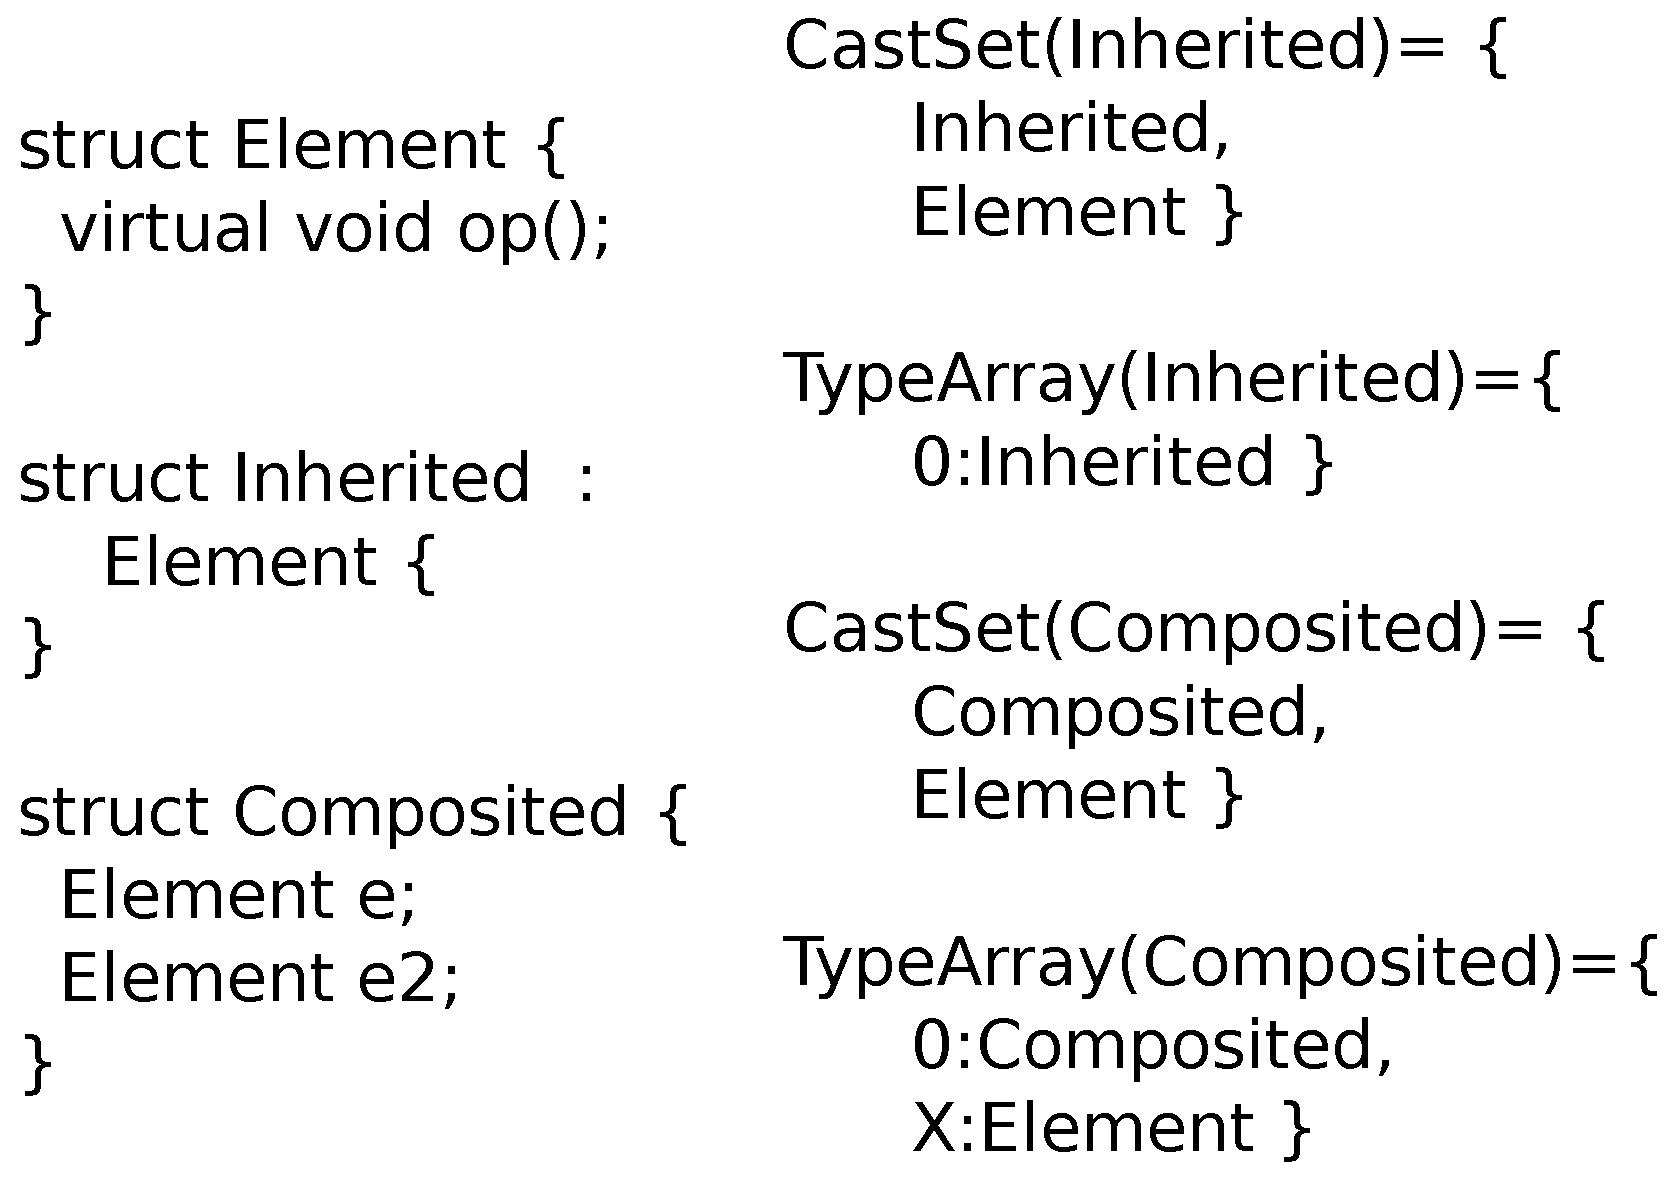
\includegraphics[width=2.8in]{figs/typeexample.eps}
  \caption{
  Example of the interaction between CastSet and TypeArray. For both inheritance and composition,
  the CastSet includes Element as the new type contains a nested Element object at offset 0. The
  TypeArrays include the type itself at offset 0,
  while including other nested types at different offsets, such as the second Element member in the case of the
  Composited class.
  }
  \label{fig:typeexample}
  \vspace{-1em}
\end{figure}

CastSets and TypeArrays are constructed at compile time and stored in global memory, with
the latter pointing to the appropriate CastSets. Type confusion detection requires that
the instrumentation identifies the base pointer of the object as well as the NestedTypeArray corresponding
to the object. This allows to system to retrieve the appropriate CastSet and to identify if the cast target
is within the allowed set or not. This information can be tracked with a simple 8 byte metadata scheme.
The first metadata corresponding to the object includes a pointer to the NestedTypeArray itself, while subsequent
metadata elements store the relative offset (negative) required to reach the base pointer of the object.
Together with the alignment information retrieved as part of the metadata retrieval process, this gives the
instrumentation all the information it needs to perform type confusion detection. Storing different types of
information in the metadata field adds additional complexity (branch for negative values), but it allows
for smaller metadata sizes and thus allocation-time overhead. For this application the 
metadata retrieval frequency is significantly reduced (only required for static down-casts),
thus we expect that this design is preferable to ensure minimal overhead.

\subsection{Dangling Pointer Detection}

Use-after-free vulnerabilities represent the most prominent attack vectors in today's browser landscape~\cite{lee2015preventing}.
While a lot of effort is invested to detect these vulnerabilities via static analysis and software testing,
they typically manifest in highly specialized contexts, making them hard to detect and to fix preemptively.
As such, a couple of systems have been suggested recently to mitigate the underlying reason for the vulnerabilities,
dangling pointers~\cite{lee2015preventing,younan2015freesentry}. These systems rely on tracking heap allocations and
their connectivity at run time. When an object is freed, the systems identify whether there are any pointers
still pointing into the object being released. These pointers are then set to a benign value of NULL to mitigate
potential memory dereferences using them.

Systems for tracking dangling pointers share an underlying design based on three core
data structures. The first is the object map, which identifies heap objects based on any pointer
into the object itself (at any offset). This is equivalent to object metadata tracking.
DangNull~\cite{lee2015preventing} uses red-black trees to track heap allocations, but as discussed
in section~\ref{sec:introduction}, this scheme is susceptible to heavy and unpredictable overhead.
FreeSentry~\cite{younan2015freesentry} uses a label based system, which is equivalent to the fixed
compression ratio metadata shadowing. This scheme offers
fast fixed-time metadata retrieval, but incurs significant allocation-time and memory overhead. In contrast,
\projectname{} combines low allocation- and  lookup overhead with efficient memory usage.

The second data structure is a pointer map, which maps locations storing pointers with information about the
pointer itself. This is essentially location-specific metadata, thus a hash table is the most appropriate
data structure (as no range lookups are required) and both systems use it. The last data structure is the collection
of pointer to object mappings. This structure is used to accumulate information about all incoming/outgoing pointer
for a particular object.  Outgoing pointers are best tracked using a red-black tree as performed in DangNull to
allow efficient retrieval of the outgoing pointer residing at a particular offset in the object. FreeSentry on the
other hand tracks only incoming pointers which can be stored in a simple linked list instead. The disadvantage of
tracking only incoming pointers, is the difficulty of inferring if the source object of the incoming pointer is
still live in memory or not.

We propose a new dangling pointer tracking scheme inspired by FreeSentry, but using \projectname{} to track
object information. The proposed scheme tracks for each heap object the head of the
incoming pointer list as well as a unique identifier to help with object liveness. For each incoming pointer
we track the identifier of the source object, its base address, the address in memory where the pointer is stored
and the pointer value itself.
A hash table is used to map memory
locations with pointers stored within. Each pointer is represented by a link to the appropriate incoming pointer
element described previously. When a pointer is stored in memory, the old incoming pointer is destroyed and a new
one is created and prepended to the list of the target object. Then a link towards this element is stored in the appropriate
hash table location. When an object is freed, the system looks up the incoming pointer list checking if any of the entries
are still valid. An entry is valid if the specified source object still resides at the specified base pointer (based on the
unique identifier) and if the pointer location still contains the specified pointer value. For all valid entries the value stored
in the pointer location is reset to NULL to ensure no use-after-free vulnerabilities can exist. Figure~\ref{fig:metasentry}
showcases the data-structures described above.

\begin{figure}[t]
\center
  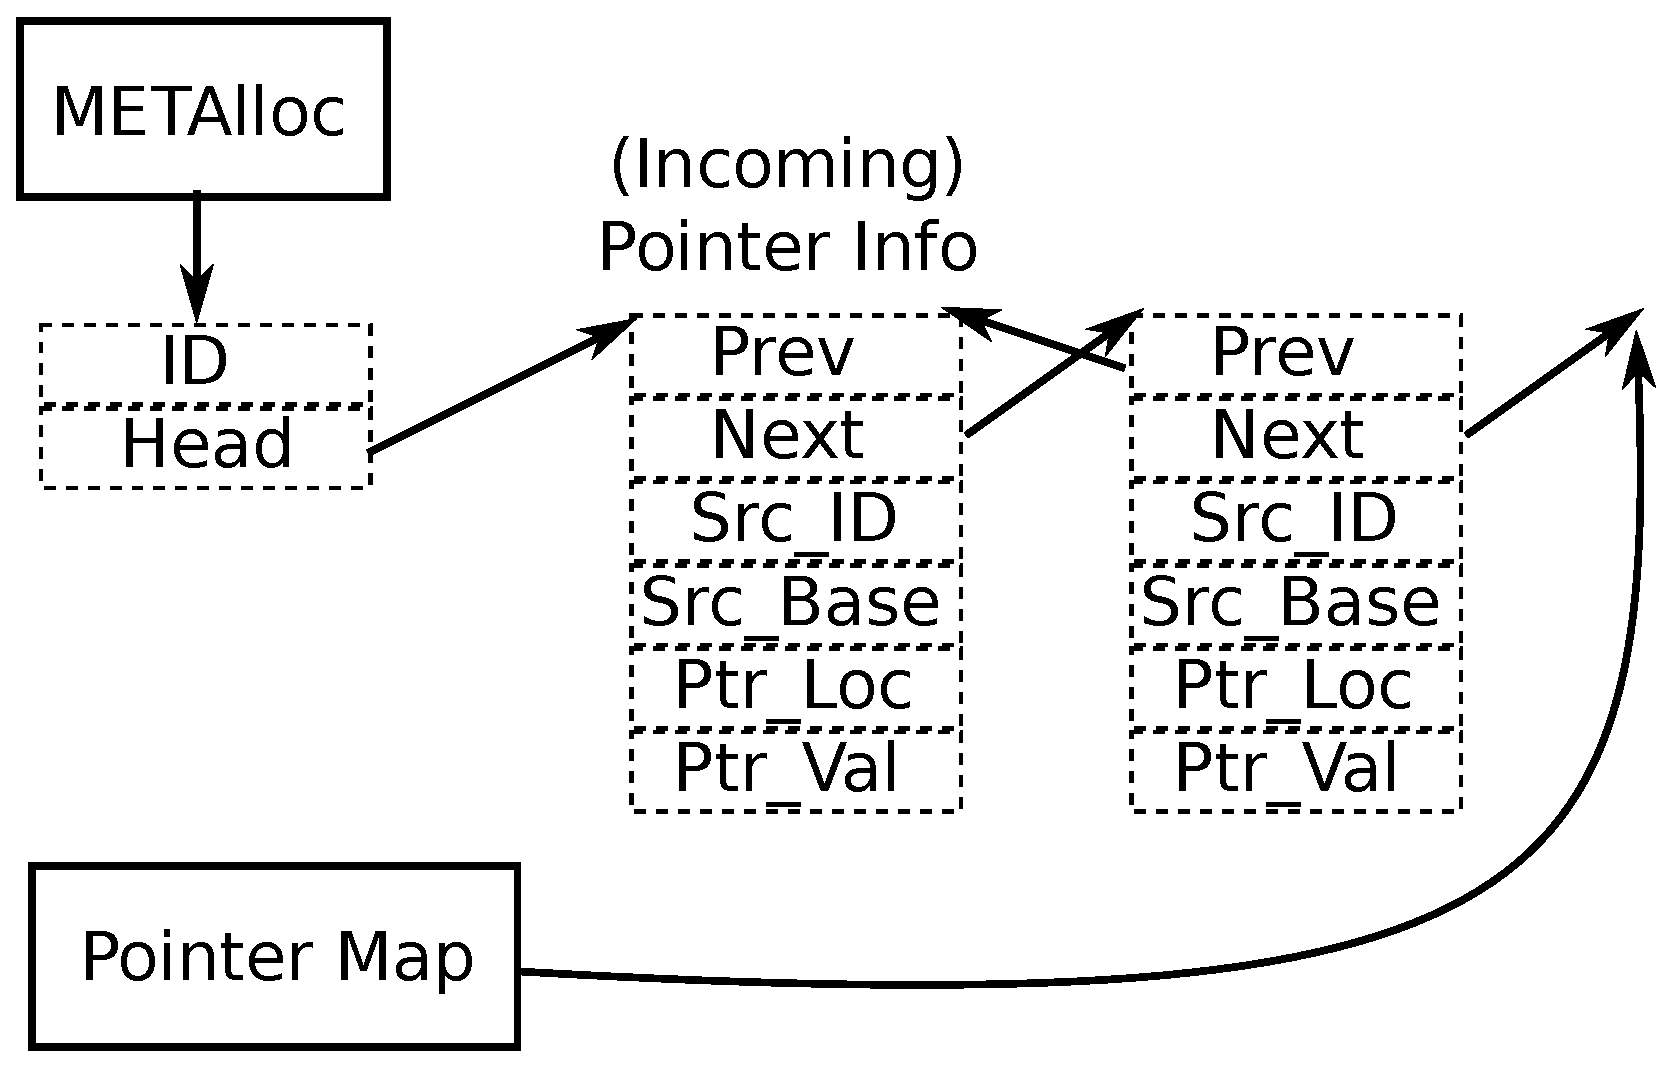
\includegraphics[width=2.8in]{figs/metasentry.eps}
  \caption{
  Data-structures used to implement dangling pointer detection using \projectname{}.
  \projectname{} allows the retreival of a unique object ID as well as a pointer to the head
  of a doubly linked list including information about incoming pointer information. The Pointer Map
  is used to retrieve the pointer infromation corresponding to a pointer stored in a given location.
  For each pointer we store information about the object containing it (ID and base address) as well
  as the location storing the pointer and the pointer value itself to allow nullification.
  }
  \label{fig:metasentry}
  \vspace{-1em}
\end{figure}
